Real analysis originates from calculus. When we were studying calculus, we deal with two sides:
differentiation and integration, which are inverse operations.
Real analysis is the study of these two sides in a more rigorous way: starting from generalizing the 
Riemann integral, but why?

Recall that when we were studying Riemann integral, we define 
$f: [a, b] \to \mathbb{R}$ as a bounded function on a closed interval $[a, b]$.
\begin{gather}
\int_a^b f(x) \, dx \text{ exists?}
\end{gather}
The Riemann integral is then defined as the limit of Riemann sums as the partition of the interval becomes finer.
We take the partition of the interval $[a, b]$ into $n$ subintervals,
$P = \{ a < x_0 < x_1 < \cdots < x_n = b \}$,
take $t_k \in [x_{k-1}, x_k]$ as a sample point in each subinterval,
and then we form the Riemann sum:
\begin{gather}
R(f, P) = \sum_{k=1}^n f(t_k) \Delta x_k
\end{gather}
where $\Delta x_k = x_k - x_{k-1}$ is the width of the $k$-th subinterval.
The Riemann integral is then defined as:
\begin{gather}
\int_a^b f(x) \, dx = \lim_{n \to \infty} R(f, P)
\end{gather}
if the limit exists.

In Darboux integral, we define the upper and lower sums:
\begin{gather}
L(f, P) = \sum_{k=1}^n m_k \Delta x_k, \quad U(f, P) = \sum_{k=1}^n M_k \Delta x_k
\end{gather}
where $m_k = \inf_{x \in [x_{k-1}, x_k]} f(x)$ and $M_k = \sup_{x \in [x_{k-1}, x_k]} f(x)$.
The Darboux integral is then defined as:
\begin{gather}
\int_a^b f(x) \, dx = \lim_{n \to \infty} L(f, P) = \lim_{n \to \infty} U(f, P)
\end{gather}
if the limit exists.
The Riemann integral and the Darboux integral are equivalent, but the Darboux integral is more general.

\begin{eg}
    \label{eg1}
    \begin{gather*}
        f(x) = \begin{cases}
            1 & \text{if } x \in \mathbb{Q} \\
            0 & \text{otherwise}
        \end{cases}
    \end{gather*}
    for $x \in [0,1].$
    The Riemann integral does not exist, but the Darboux integral exists and is equal to 0.
    \begin{gather*}
        L(f, P) = 0, \quad U(f, P) = 1
    \end{gather*}
\end{eg}

Lebesgue extends the idea of Riemann integral to more general functions.
\begin{theorem}[Lebesgue's Criterion for Integrability]
    \

    Set $\mathcal{D} = \{ x \in [a,b] | f \text{ is not continuous at } x\}.$
    Let $f: [a, b] \to \mathbb{R}$ be a bounded function. Then $f$ is Lebesgue is integrable if and only if $\mathcal{D}$ is of measure zero.
\end{theorem}

We first show the difference of Riemann integral and Darboux integral in the graph(left).
Then let's look back at example \ref{eg1} (right), we can see that the function is not continuous at any point in $[0,1]$.
By the definition of Riemann integral, we can see that the Riemann integral does not exist.

\tikzset{every picture/.style={line width=0.75pt}} %set default line width to 0.75pt        
\begin{tikzpicture}[x=0.75pt,y=0.75pt,yscale=-1,xscale=1]
%uncomment if require: \path (0,300); %set diagram left start at 0, and has height of 300
\centering
%Shape: Axis 2D [id:dp5480263477292685] 
\draw  (50,241.64) -- (303.8,241.64)(75.38,53) -- (75.38,262.6) (296.8,236.64) -- (303.8,241.64) -- (296.8,246.64) (70.38,60) -- (75.38,53) -- (80.38,60) (95.38,236.64) -- (95.38,246.64)(115.38,236.64) -- (115.38,246.64)(135.38,236.64) -- (135.38,246.64)(155.38,236.64) -- (155.38,246.64)(175.38,236.64) -- (175.38,246.64)(195.38,236.64) -- (195.38,246.64)(215.38,236.64) -- (215.38,246.64)(235.38,236.64) -- (235.38,246.64)(255.38,236.64) -- (255.38,246.64)(275.38,236.64) -- (275.38,246.64)(55.38,236.64) -- (55.38,246.64)(70.38,221.64) -- (80.38,221.64)(70.38,201.64) -- (80.38,201.64)(70.38,181.64) -- (80.38,181.64)(70.38,161.64) -- (80.38,161.64)(70.38,141.64) -- (80.38,141.64)(70.38,121.64) -- (80.38,121.64)(70.38,101.64) -- (80.38,101.64)(70.38,81.64) -- (80.38,81.64) ;
\draw   ;
%Curve Lines [id:da5750477268932044] 
\draw [line width=0.75] [line join = round][line cap = round]   (95.8,173.6) .. controls (103.93,144.95) and (123.8,114.2) .. (153.8,110.6) .. controls (177.8,108.6) and (188.85,138.59) .. (213.8,132.6) .. controls (231.8,128.28) and (258.92,107.8) .. (275.8,115.4) ;
%Straight Lines [id:da7177706943638141] 
\draw  [dash pattern={on 0.84pt off 2.51pt}]  (275.8,115.4) -- (275.8,242.6) ;
%Shape: Rectangle [id:dp5408053767416018] 
\draw  [fill={rgb, 255:red, 245; green, 166; blue, 35 }  ,fill opacity=0.38 ] (95.8,241.6) -- (115.8,241.6) -- (115.8,173.6) -- (95.8,173.6) -- cycle ;
%Shape: Rectangle [id:dp3923239636084771] 
\draw  [fill={rgb, 255:red, 208; green, 2; blue, 27 }  ,fill opacity=0.33 ] (95.8,132.6) -- (115.8,132.6) -- (115.8,173.6) -- (95.8,173.6) -- cycle ;
%Shape: Rectangle [id:dp24584912849228258] 
\draw   (174.8,129.6) -- (194.8,129.6) -- (194.8,241.6) -- (174.8,241.6) -- cycle ;
%Shape: Rectangle [id:dp34691668964713374] 
\draw   (174.8,117.6) -- (194.8,117.6) -- (194.8,129.6) -- (174.8,129.6) -- cycle ;
%Shape: Axis 2D [id:dp40737828571320833] 
\draw  (333,238.64) -- (586.8,238.64)(358.38,50) -- (358.38,259.6) (579.8,233.64) -- (586.8,238.64) -- (579.8,243.64) (353.38,57) -- (358.38,50) -- (363.38,57)  ;
%Shape: Rectangle [id:dp28240967807166417] 
\draw   (442.8,126.6) -- (462.8,126.6) -- (462.8,238.6) -- (442.8,238.6) -- cycle ;
%Straight Lines [id:da2779504540997346] 
\draw [color={rgb, 255:red, 245; green, 166; blue, 35 }  ,draw opacity=1 ]   (442.8,126.6) -- (462.8,126.6) ;

% Text Node
\draw (280,98) node [anchor=north west][inner sep=0.75pt]  [font=\footnotesize] [align=left] {$\displaystyle f( x)  >0$};
% Text Node
\draw (272,247) node [anchor=north west][inner sep=0.75pt]  [font=\footnotesize] [align=left] {$\displaystyle b$};
% Text Node
\draw (96,246) node [anchor=north west][inner sep=0.75pt]  [font=\footnotesize] [align=left] {$\displaystyle a$};
% Text Node
\draw (425,72) node [anchor=north west][inner sep=0.75pt]  [font=\footnotesize] [align=left] {$\displaystyle f( x) \ =\ \begin{cases}
1 & x\in Q\\
0 & otherwise
\end{cases}$};
% Text Node
\draw (555,244) node [anchor=north west][inner sep=0.75pt]  [font=\footnotesize] [align=left] {$\displaystyle b$};
% Text Node
\draw (379,243) node [anchor=north west][inner sep=0.75pt]  [font=\footnotesize] [align=left] {$\displaystyle a$};

\draw   (273.8,241.64) -- (277.8,241.64)(275.8,239.64) -- (275.8,243.64) ;
\end{tikzpicture}

What do we really want by taking integrals?
Basically speaking, we want to find the area under the curve.
In the case of Riemann and Darboux integrals,
we partitioned the $x$-axis into subintervals,
but we encountered problems.

It's quite common that we start to try partitioning the $y$-axis instead.
We define the Lebesgue measure as
$E_{\lambda} = \left\{ x \in [a,b] | f(x) > \lambda \right\}.$

\tikzset{every picture/.style={line width=0.75pt}} %set default line width to 0.75pt        

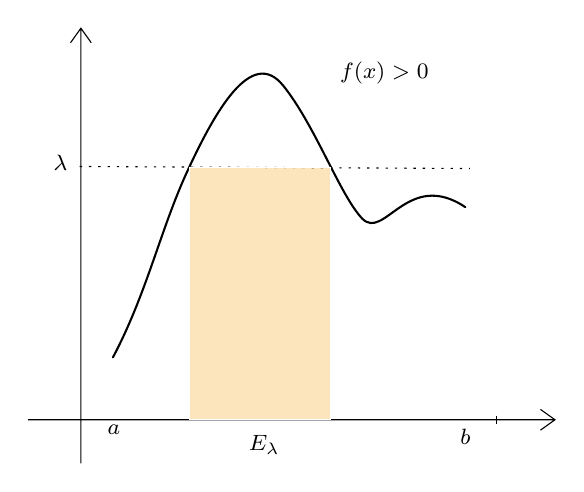
\begin{tikzpicture}[x=0.75pt,y=0.75pt,yscale=-1,xscale=1]
%uncomment if require: \path (0,300); %set diagram left start at 0, and has height of 300

%Shape: Axis 2D [id:dp7368713459977554] 
\draw  (50,241.64) -- (303.8,241.64)(75.38,53) -- (75.38,262.6) (296.8,236.64) -- (303.8,241.64) -- (296.8,246.64) (70.38,60) -- (75.38,53) -- (80.38,60)  ;
%Curve Lines [id:da47596783152208033] 
\draw [line width=0.75] [line join = round][line cap = round]   (90.8,211.6) .. controls (107.26,180.5) and (113.8,149.6) .. (126.8,121.6) .. controls (139.8,93.6) and (157.48,61.62) .. (172.8,80.6) .. controls (188.12,99.58) and (200.18,133.32) .. (210.8,144.6) .. controls (221.42,155.88) and (232.8,120.6) .. (260.6,139.2) ;
%Straight Lines [id:da5789424259496938] 
\draw  [dash pattern={on 0.84pt off 2.51pt}]  (74.8,119.6) -- (262.8,120.6) ;
%Straight Lines [id:da9105862457970941] 
\draw  [dash pattern={on 0.84pt off 2.51pt}]  (127.8,119.6) -- (127.8,241.6) ;
%Straight Lines [id:da6325422272939283] 
\draw  [dash pattern={on 0.84pt off 2.51pt}]  (195.8,119.6) -- (195.8,241.6) ;
%Shape: Rectangle [id:dp20836883762828573] 
\draw  [color={rgb, 255:red, 255; green, 255; blue, 255 }  ,draw opacity=1 ][fill={rgb, 255:red, 245; green, 166; blue, 35 }  ,fill opacity=0.3 ] (127.8,120.1) -- (195.8,120.1) -- (195.8,241.6) -- (127.8,241.6) -- cycle ;

% Text Node
\draw (257,245) node [anchor=north west][inner sep=0.75pt]  [font=\footnotesize] [align=left] {$\displaystyle b$};
% Text Node
\draw (87,243) node [anchor=north west][inner sep=0.75pt]  [font=\footnotesize] [align=left] {$\displaystyle a$};
% Text Node
\draw (61,113) node [anchor=north west][inner sep=0.75pt]  [font=\footnotesize] [align=left] {$\displaystyle \lambda $};
% Text Node
\draw (155,248) node [anchor=north west][inner sep=0.75pt]  [font=\footnotesize] [align=left] {$\displaystyle E_{\lambda }$};
% Text Node
\draw (199,68) node [anchor=north west][inner sep=0.75pt]  [font=\footnotesize] [align=left] {$\displaystyle f( x)  >0$};

\draw   (273.8,241.64) -- (277.8,241.64)(275.8,239.64) -- (275.8,243.64) ;
\end{tikzpicture}

Assuming that $E_{\lambda}$ is measurable, we know that the shaded area is $\lambda \vert E_{\lambda} \vert.$

